\section{Semáforos}

	Muestre la pantalla de compilación y ejecución de los programas proceso1.c y proceso2.c, ejecutelos en el orden anterior

	\begin{center}
		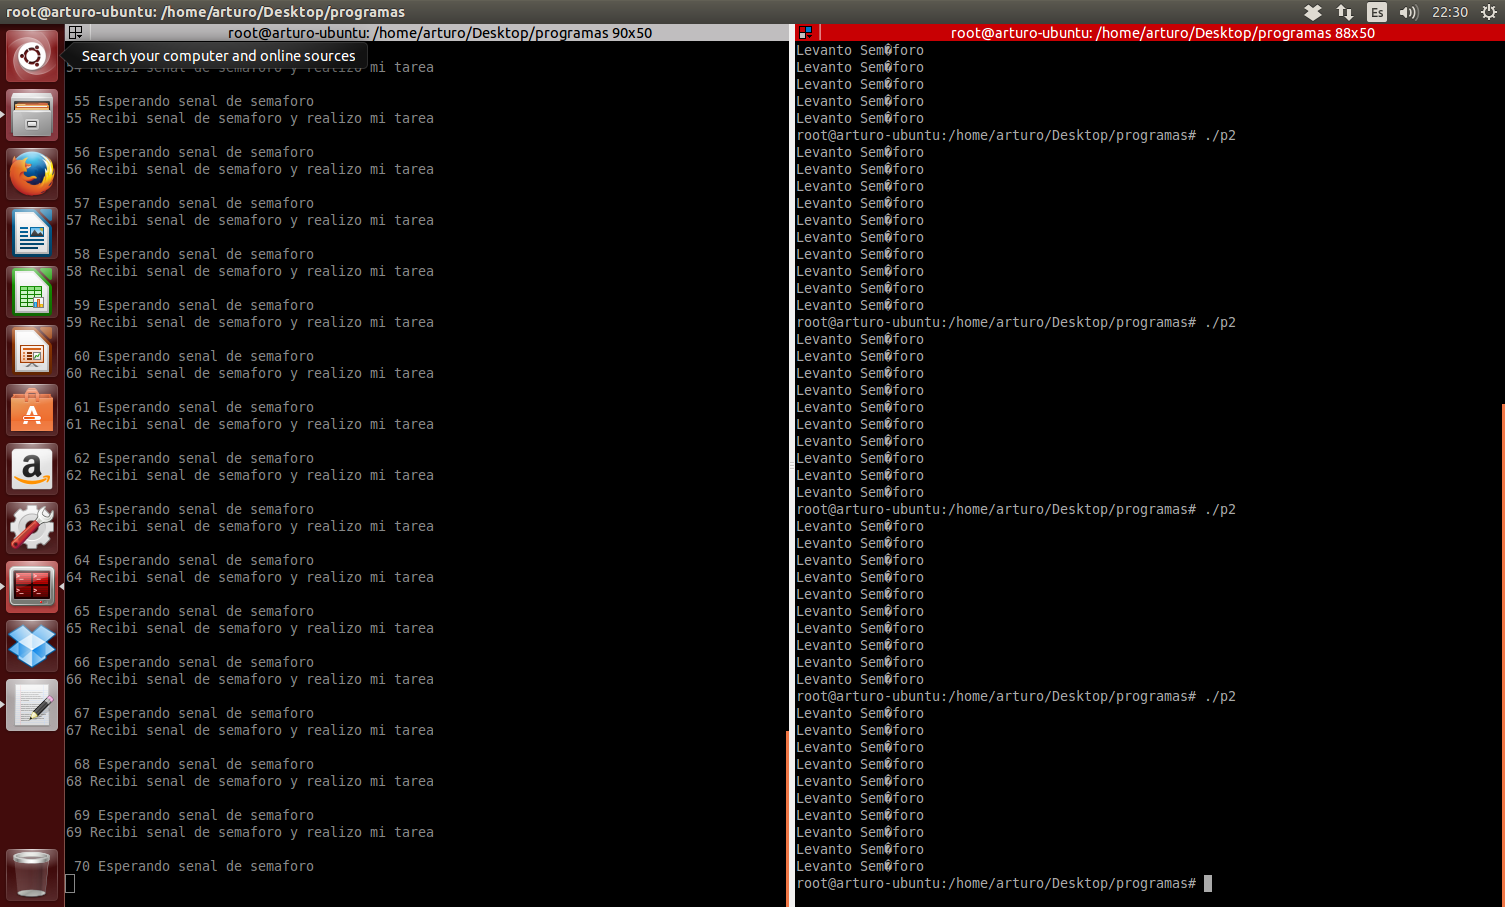
\includegraphics[width=\linewidth]{imagenes/pic.png}
	\end{center}

Investigue lo siguiente:

\begin{itemize}
    \item Escriba el nombre de la biblioteca donde estan definidas los siguientes elementos: struct semid\_ds, struct seminfo, semget, semop y semctl.
    \begin{tcolorbox}
        \textit{sys/sem.h}
    \end{tcolorbox} 
    \item Describa qué es lo que realizan las funciones ftok, shmget, shmat y shmctl, además de describir sus argumentos de entrada y la salida que proporcionan
    \begin{tcolorbox}
	\begin{itemize}
		\item \textbf{ftok}\\
		Genera una llave System V IPC de un nombre de ruta y un identificador de proyecto. Esto es:
		\begin{itemize}
			\item Parámetros
			\begin{itemize}
				\item \textbf{const char *}\textit{pathname}\\
			El nombre de ruta.
				\item \textbf{int} \textit{proj\_id}\\
			El identificador de proyecto.
			\end{itemize}
			\item Salida \textbf{key\_t}\\
			La llave resultante.
		\end{itemize}
		\item \textbf{shmget}\\
		Crea un segmento de memoria compartido.
		\begin{itemize}
			\item Parámetros
			\begin{itemize}
				\item \textbf{key\_t }\textit{key}\\
			La llave a utilizar IPC.
				\item \textbf{size\_t } \textit{size}\\
			El tamaño de la memoria asignada.
				\item \textbf{int} \textit{shmflag}\\
			Instrucción que especifica que acción se debe realizar. Por ejemplo, IPC\_CREAT creará el nuevo segmento, mientras que IPC\_EXCL hará que la función falle si ya existe ese segmento de memoria.
			\end{itemize}
			\item Salida \textbf{int}\\
			El identificador de memoria compartida. Si tiene valor -1, esta función falló. (Error específicado con errno)
		\end{itemize}
	\end{itemize}
    \end{tcolorbox}
    \begin{tcolorbox}
    \begin{itemize}
    \item \textbf{shmat}\\
    Maneja las operaciones de memoria compartida.
	\begin{itemize}
		\item Parámetros
		\begin{itemize}
			\item \textbf{int} \textit{shmid}\\
		El identificador de memoria compartida a utilizar.
			\item \textbf{const void *}\textit{shmaddr}\\
		La dirección donde se relacionará la memoria compartida con los datos del proceso.
			\item \textbf{int} \textit{shmflg}\\
		Bandera para especificar la operación.
		\end{itemize}
		\item Salida \textbf{void}\\
		-1 si ha habido error.
	\end{itemize}
	\item \textbf{shmctl}\\
	Controla la memoria compartida.
	\begin{itemize}
		\item Parámetros
		\begin{itemize}
			\item \textbf{int} \textit{shmid}\\
		El identificador de memoria compartida a utilizar.
			\item \textbf{int} \textit{cmd}\\
		Se especifica el comando.
			\item \textbf{struct shmid\_ds *}\textit{buf}\\
		Estructura que específica los datos a utilizar para un comando dado.
		\end{itemize}
		\item Salida \textbf{int}\\
		Dependiente del comando utilizado. -1 si hubo error.
	\end{itemize}
    \end{itemize}
    \end{tcolorbox}
\end{itemize}